%% LaTeX Beamer presentation template (requires beamer package)
\documentclass{beamer}
 
\mode<presentation>
{
  \usetheme[compress]{FH-DO}
  \setbeamercovered{transparent}
}


\usepackage[german]{babel}
\usepackage[latin1]{inputenc}
\usepackage{xcolor,cancel,pifont,enumerate,tcolorbox}
\usepackage{pgfgantt,changepage,tikz}

%% This is needet for formula like normal TeX and \mathcal
\usefonttheme[onlymath]{serif}

%% Cancel stuff in red
\newcommand\hcancel[2][black]{\setbox0=\hbox{$#2$}%
  \rlap{\raisebox{.45\ht0}{\textcolor{#1}{\rule{\wd0}{1pt}}}}#2}
%% For img caption numbered


%% fancy crossmark and checkmark
\newcommand{\xmark}{\ding{55}}
\newcommand{\cmark}{\ding{51}}

% font definitions, try \usepackage{ae} instead of the following
% three lines if you don't like this look
% \usepackage{mathptmx}
\usepackage[scaled=.90]{helvet}
\usepackage{courier}
\usepackage[font=scriptsize]{caption}

\usepackage[T1]{fontenc}


\usepackage{comment}
%usepackage{appendixnumberbeamer}
\usepackage{amsmath}
\usepackage{pgfpages}
% citations
%\usepackage{natbib}
%\bibpunct{(}{)}{;}{a}{,}{,}
%\def\citeapos#1{\citeauthor{#1}'s (\citeyear{#1})}
%\renewcommand{\bibsection}{\subsubsection*{\bibname }}
\title{Autoencoder}
\subtitle{Denoising und Anomaliedetektion von Audiodaten}
%\titlegraphic{}

\author{Timo Grautst\"uck}
% - Use the \inst command only if there are several affiliations.
% - Keep it simple, no one is interested in your street address.
\institute[FH-DO]
{
  Fachhochschule-Dortmund \\
  FB: Informationstechnik \\
  \texttt{timo.grautstueck@fh-dortmund.de}
}

\date{\small{\today}}


% This is only inserted into the PDF information catalog. Can be left
% out.
%\subject{Subject}



% If you have a filex called "university-logo-filename.xxx", where xxx
% is a graphic format that can be processed by latex or pdflatex,
% resp., then you can add a logo as follows:

% Delete this, if you do not want the table of contents to pop up at
% the beginning of each subsection:
%\AtBeginSubsection[]
% {
% \begin{frame}<beamer>
% \frametitle{Outline}
% \tableofcontents[currentsection,currentsubsection]
%\end{frame}
%}

% If you wish to uncover everything in a step-wise fashion, uncomment
% the following command:

%\beamerdefaultoverlayspecification{<+->}

\begin{document}

\begin{frame}
  \titlepage
\end{frame}

\begin{frame}
  \frametitle{Wor�ber wollen wir sprechen ?}
  \tableofcontents
\end{frame}

\section{Einf\"uhrung}

\begin{frame}
  \frametitle{Autoencoder ?}
  \begin{minipage}{0.34\textwidth}
    \vspace{0.3cm}
    \begin{figure}[h]
      \begin{tikzpicture} [auto,node distance=1.3cm,semithick]
        \tikzstyle{bubble}=[circle, fill=gray!20, draw, inner sep = 0mm, minimum size = 6mm]
        \node[bubble] (Input) {\scriptsize{$\boldsymbol{x}$}};
        \node[bubble] (Code) [above right of = Input] {\scriptsize{$\boldsymbol{h}$}};
        \node[bubble] (Recon) [below right of = Code] {\scriptsize{$\boldsymbol{r}$}};
        
        \path[->,>=stealth,shorten >=1pt, shorten <= 1pt]
        (Input) edge node{\scriptsize{$f$}} (Code) 
        (Code) edge node{\scriptsize{$g$}}(Recon);
      \end{tikzpicture}
      \caption{Autoencoder Struktur}
    \end{figure}
  \end{minipage}
  \hfill
  \begin{minipage}{0.6\textwidth}
    \begin{block}{\textbf{Notation}}
      \begin{itemize}
      \item $\boldsymbol{x} \rightarrow$ originaler Input
      \item $\boldsymbol{h}=f(\boldsymbol{x}) \rightarrow$ latente Repr\"asentation
      \item $\boldsymbol{r}= g(\boldsymbol{h})\rightarrow$ rekonstruierter Input
      \item $f \rightarrow$ Encoder
      \item $g \rightarrow$ Decoder
      \end{itemize}
    \end{block}
  \end{minipage}
  \begin{block}{\textbf{Aufgabe}}
    \begin{itemize}
    \item Kopiere den Input zu einem Output $\Rightarrow x = g(f(\boldsymbol{x}))$ \textcolor{red}{\xmark} 
    \item Kopiere den Input zu einem Output, sodass $\boldsymbol{h}$ n�tzliche Eigenschaften lernt $\Rightarrow x \approx g(f(\boldsymbol{x}))$ \textcolor{green}{\cmark}
    \end{itemize}
  \end{block}
\end{frame}

\subsection{Autoencoder}
\begin{frame}
  \frametitle{Wie k�nnen wir das erreichen ?}
  \begin{block}{\textbf{K�nstlichen Neuronalen Netzen \textit{(ANN's)}}}
    Eine einfache Form eines Autoencoders w�re ein Multilayer Perceptron \textit{(MLP)}, in welchen Eingabe- sowie Ausgabeschicht die gleiche Anzahl an Neuronen enthalten und die Hiddenlayers ein sogenanntes \textit{bottleneck} bilden. Hierzu k�nnen auch Convolutional Layers genutzt werden.
  \end{block}
  \begin{minipage}{0.5\textwidth}
    \begin{block}{\textbf{Verschiedene Arten von AE}}
      \begin{enumerate}
      \item Undercomplete Autoencoder
        \begin{itemize}
        \item $\mathcal{L}(\boldsymbol{x},g(f(\boldsymbol{x})))$
        \end{itemize} 
      \item Sparse Autoencoder
        \begin{itemize}
        \item $\mathcal{L}(\boldsymbol{x},g(f(\boldsymbol{x})))+\Omega(\boldsymbol{h})$ 
        \end{itemize}
      \end{enumerate}
    \end{block}
  \end{minipage}
  \hfill
  \begin{minipage}{0.45\textwidth}
    \begin{figure}
      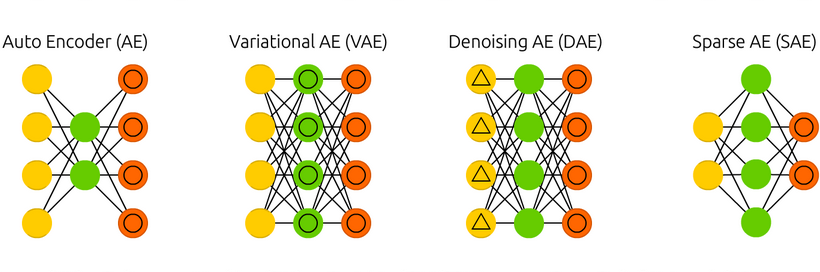
\includegraphics[width=5.5cm]{img/Autoencoder.png}
      \caption*{\tiny{\textbf{Quelle:} \url{https://www.asimovinstitute.org/neural-network-zoo/}}}
      \end{figure}
  \end{minipage}
\end{frame}


\subsection{}
\begin{frame}
  \frametitle{Denoising Autoencoder}
  \begin{figure}
    \centering
    \begin{tikzpicture}
      \tikzstyle{arrow} = [->,>=stealth,shorten >=1pt,shorten <=1pt,thick]
      \tikzstyle{bendarrow} = [bend right = 45,->,>=stealth,shorten >=1pt,shorten <=1pt]
      \node[inner sep=0pt] (audio) at (-2.7,-2.2) {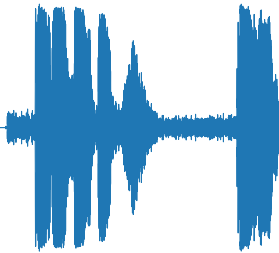
\includegraphics[width=.15\textwidth]{img/audio.png}};
      \node[inner sep=0pt] (noise) at (-2.7,-4) {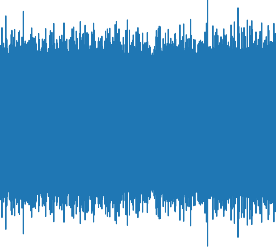
\includegraphics[width=.15\textwidth]{img/noise.png}};%
       \node[inner sep=0pt] (audionoise) at (3.8,-3) {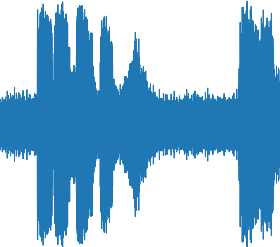
\includegraphics[width=.15\textwidth]{img/noisy_signal.png}};
      \node (add) [circle,draw,inner sep = 0pt, minimum size=4mm,thick] at (-1.2,-3){+};
      \draw[thick] (-0.5,-2) -- (-0.5,-4) -- (0.5,-3.5) -- (0.5,-2.5) -- (-0.5,-2);
      \draw[thick] (2.5,-2) -- (2.5,-4) -- (1.5,-3.5) -- (1.5,-2.5) -- (2.5,-2);
      \draw[arrow] (audio) -- (add);
      \draw[arrow] (noise) -- (add);
      \draw[arrow] (add) -- (-0.5,-3);
      \node[rectangle,draw,align=center,minimum width = 0.8cm,minimum height =0.8cm,thick,fill = gray!30] (bottleneck) at (1,-3){$\boldsymbol{h}$};
      \node at (0,-3) {\scriptsize{Encoder}};
      \node at (2,-3) {\scriptsize{Decoder}};
      \node at (1,-3.8) {\scriptsize{Bottleneck}};
      \draw[arrow] (2.5,-3) -- (audionoise);
      \path[<->,>=stealth,shorten >=1pt,shorten <=2pt,thick] (audionoise.north) edge[bend right = 35,dashed] node[below,yshift=-0.2cm,xshift = -0.3cm] {\scriptsize{Rekonstruktionsverlust}} (audio);
    \end{tikzpicture}
    \caption{Denoising Autoencoder \textit{(DAE)}}
  \end{figure}
  $$\boxed{\mathcal{L}(\boldsymbol{x},g(f(\boldsymbol{\tilde{x}})))}$$
    \begin{center}$\boldsymbol{\tilde{x}}$ ist eine Kopie von $\boldsymbol{x}$, mit additivem Rauschen.\end{center}
\end{frame}

\subsection{Software/Bibliotheken}
\begin{frame}
  \frametitle{Software/Tools}
  \hspace{-0.3cm}
  \begin{minipage}{0.3\textwidth}
    \begin{figure}
      \centering
      
\includegraphics[width=2.5cm]{img/tensorflow.png}
      \caption{TensorFlow}
    \end{figure}
    \begin{figure}
      \centering
      
\includegraphics[width=1.5cm]{img/jupyter.png}
      \caption{Jupyter}
    \end{figure}
  \end{minipage}
  \hfill
  \begin{minipage}{0.2\textwidth}
    \begin{figure}
      \centering
      
\includegraphics[width=1.5cm]{img/python.png}
      \caption{Python}
    \end{figure}
  \end{minipage}
  \hfill
  \vspace{-0.2cm}
  \begin{minipage}{0.3\textwidth}
    \begin{figure}
      \centering
      
\includegraphics[width=1.9cm]{img/keras.png}
      \caption{Keras}
    \end{figure}
    \begin{figure}
      \centering
      
\includegraphics[width=3.5cm]{img/librosa.png}
      \caption{Librosa}
    \end{figure}
  \end{minipage}
\end{frame}

\section{Agenda}
%%-Gantt-Diagramm-%%
\subsection{Zeitplan}
\begin{frame}
  \frametitle{Zeitplan}
  \begin{adjustwidth}{-1.7cm}{-1cm}
    \begin{figure}[h]
      \centering
      \begin{ganttchart}[
          vgrid, time slot format=isodate-yearmonth, time slot unit=month,
          y unit chart= 0.7cm, y unit title = 0.6cm,
          %% Setting for Group
          group right shift = -0.1, group left shift = 0.1, group/.append style={fill=black!50,draw = black},
          group peaks tip position=0, group peaks height=.08, group height =.3,
          %% Settings for Milestone
          milestone left shift = 0.7, milestone right shift = 0.3,
          %% Settings for bars
          bar top shift = .2,
        ]{2021-08}{2023-02}
        \gantttitlecalendar{year, month} \\
        \ganttgroup[inline,group right shift = 0.3]{\scriptsize{EipA}}{2021-08}{2021-08}
        \ganttgroup[inline,group left shift = 0.45]{\scriptsize{Projektarbeit 1}}{2021-9}{2022-02}
        \ganttgroup[
          inline,group label font=\color{gray!80!black}
        ]{\scriptsize{Auslands-/Praxissemester}}{2022-03}{2022-07}
        \ganttgroup[inline]{\scriptsize{PA2/Bachelorarbeit}}{2022-08}{2023-01}\\
        \ganttbar[inline, bar/.append style={fill=red!50},bar left shift = 0.7,bar right shift = 0.1]{\scriptsize{\textit{WS 2021/22}}}{2021-09}{2022-01}
        \ganttbar[inline, bar/.append style={fill=red!50},bar left shift = 0.7,bar right shift = -0.5]{\scriptsize{\textit{SoSe 2022}}}{2022-03}{2022-07} 
        \ganttbar[inline, bar/.append style={fill=red!50},bar left shift = 0.6,bar right shift = 0.1]{\scriptsize{\textit{WS 2022/23}}}{2022-09}{2023-01}
        \\
        %% Milestones %%
        \ganttmilestone[milestone right shift = 0.6, milestone left shift = 1.0]{}{2021-08}
        \ganttmilestone{}{2022-02}
        \ganttmilestone{}{2023-01}
        \\
        %% Bars %%
        \ganttbar[bar left shift = 0.3, bar right shift = -0.2,bar/.append style={fill=yellow!20}]{\scriptsize{Datenbeschaffung}}{2021-09}{2021-09}\\
        \ganttbar[bar/.append style={fill=green!20}]{\scriptsize{Daten untersuchen}}{2021-10}{2021-11}
        \ganttbar[bar/.append style={fill=green!20}]{}{2022-08}{2022-08}\\
        \ganttbar[bar/.append style={fill=purple!20}]{}{2021-12}{2022-01}
        \ganttbar[bar/.append style={fill=purple!20}]{\scriptsize{Modelle entwickeln}}{2022-09}{2022-11}\\ 
        \ganttbar[bar right shift = -0.2,bar/.append style={fill=blue!20}]{}{2022-01}{2022-02}
        \ganttbar[bar right shift = -0.2,bar/.append style={fill=blue!20}]{\scriptsize{TeXen}}{2022-11}{2023-01}
        %% Links %% 
        \ganttlink{elem7}{elem10}
        \ganttlink{elem10}{elem11}
        \ganttlink{elem11}{elem13}
        \ganttlink{elem15}{elem8}
        \ganttlink{elem12}{elem14}
        \ganttlink{elem16}{elem9}
      \end{ganttchart}
      \caption{Gantt-Diagramm Projekt-/Bachelorarbeit}    
    \end{figure}
  \end{adjustwidth}
\end{frame}


\subsection{Projektarbeit 1}
\begin{frame}
  \frametitle{Projektplan Arbeit 1}
  \begin{minipage}{0.45\textwidth}
    \begin{block}{\textbf{1. Datenbeschaffung}}
      \begin{itemize}
      \item Wieviel Speicherplatz ?
      \item Local vs. Cloud
      \item Kopien erstellen 
      \end{itemize}
    \end{block}
    \pause
     \begin{block}{\textbf{2. Daten untersuchen}}
      \begin{itemize}
      \item Visualisieren
      \item Auf-/Vorverarbeiten
      \item Bereinigen 
      \end{itemize}
     \end{block}
  \end{minipage}  
  \hfill
  \begin{minipage}{0.45\textwidth}
    \pause
    \begin{block}{\textbf{3. Modelle entwickeln}}
      \begin{itemize}
      \item Vergleichen 
      \item Validieren 
      \item Optimieren
      \end{itemize}
    \end{block}
    \pause
    \begin{block}{\textbf{4. TeXen}}
      \begin{itemize}
      \item Dokumentation
      \item Pr�sentation
      \end{itemize}
    \end{block}
  \end{minipage}
\end{frame}

\begin{frame}
  \frametitle{Was fehlt in der Planung ?}
  \begin{alertblock}{Probleme}
    \begin{itemize}
    \item GIGO \textit{(Garbage In, Garbage Out)}
    \item Over-/Underfitting
    \item zu wenig Daten 
    \end{itemize}
  \end{alertblock}
  \begin{exampleblock}{\textbf{Research}}
    Kein spezifischen Zeitraum in den Projekten eingeplant, immer dann wenn Research ben�tigt wird oder freie Zeitr�ume anstehen. \\
    Verst�rkt vor der Dokumentation auch im Prozess des Entwickelns \textit{(Docs, Papers, \dots)}.
  \end{exampleblock}
\end{frame}

\subsection{PA2/Bachelorarbeit}
\begin{frame}
  \frametitle{The Future}
  \begin{figure}
    \centering
    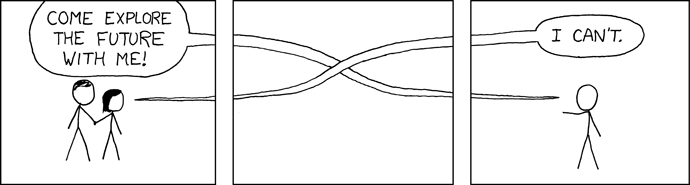
\includegraphics[width=10cm]{img/future.png}
    \caption*{\textbf{Quelle:} Randall Munroe, \url{https://xkcd.com/338/}}
  \end{figure}
\end{frame}

\begin{frame}
  \frametitle{PA2/Bachelorarbeit}
  \begin{block}{\textbf{M�gliches Vorgehen}}
    Weitere Experimente durchf�hren, weitere Modelle entwickeln, verschiedene Hyperparameter und Aktivierungsfunktionen auswerten.
    Fokus auf Vergleichen der Modelle, warum funktioniert genau dieses Modell besser als andere ? $\rightarrow$ Research  
  \end{block}
  \pause
  \begin{block}{\textbf{Daten untersuchen}}
    M�gliche Experimente:
    \begin{itemize}
    \item Frequenzbereich
    \item Fenstern
    \item Spektogram
    \end{itemize}
  \end{block}
\end{frame}


%% Tell them what they have learned
\section{Zusammenfassung}
\begin{frame}
  \frametitle{Was ich Ihnen zeigen wollte}
  \begin{enumerate}
    \item Angefangen ins Thema einzuarbeiten
      \begin{itemize}
      \item Autoencoder inkl. Arten
      \item Software/Tools
      \end{itemize}
      \pause
    \item Gedanken zur Planung der Projekte gemacht
      \begin{itemize}
      \item Gantt-Diagramm inkl. Arbeitspakete
      \end{itemize}
      \pause
    \item Hat schonmal \LaTeX \, genutzt  
      \begin{itemize}
      \item Pr�sentation / Grafiken 
      \end{itemize}
  \end{enumerate}
\end{frame}

\begin{frame}
  \begin{center}
    \begin{tabular}{cccc}
      \includegraphics[page=3, width=0.2\textwidth]{img/End.pdf}&
      \includegraphics[page=4, width=0.2\textwidth]{img/End.pdf}&
      \includegraphics[page=5, width=0.2\textwidth]{img/End.pdf}&
      \includegraphics[page=6, width=0.2\textwidth]{img/End.pdf}\\

      \includegraphics[page=7, width=0.2\textwidth]{img/End.pdf}&
      \includegraphics[page=11, width=0.2\textwidth]{img/End.pdf}&
      \includegraphics[page=12, width=0.2\textwidth]{img/End.pdf}&
      \includegraphics[page=13, width=0.2\textwidth]{img/End.pdf}\\
    \end{tabular}
    \begin{tabular}{ccc}
      \includegraphics[page=15, width=0.2\textwidth]{img/End.pdf}&
      \includegraphics[page=18, width=0.2\textwidth]{img/End.pdf}&
      \includegraphics[page=19, width=0.2\textwidth]{img/End.pdf}\\
    \end{tabular}
  \end{center}
  \begin{block}{}
    \centering Danke f�r Ihre Aufmerksamkeit.\\
    Gibt es Fragen ?
  \end{block}
\end{frame}

\begin{frame}
  \frametitle{Quellen}
  \begin{thebibliography}{}
    \setbeamertemplate{bibliography item}[book]
    \scriptsize{
    \bibitem[Goodfellow, 2016]{Goodfellow2016}\textcolor{red}{I.~Goodfellow, Y.~Bengio, A.~Courville}
      \newblock Deep Learning
      \newblock {\em MIT Press, 2016}
      \newblock \url{http://www.deeplearningbook.org}
    \bibitem[A. Geron]{Geron2019} \textcolor{red}{A.~G{\'e}ron}
      \newblock Hands-On Machine Learning with Scikit-Learn, Keras, and TensorFlow, 2nd Edition
      \newblock {\em O'Reilly Media, Inc., 2019}
      \newblock \textbf{ISBN: }{9781492032649}
      \setbeamertemplate{bibliography item}[article]
    \bibitem[D.Bank, 2020]{Bank2020} \textcolor{red}{D.~Bank, N. Koenigstein, R. Giryes}
      \newblock Autoencoders
      \newblock {\em arXiv:2003.05991, 2020}
      \newblock \url{https://arxiv.org/abs/2003.05991}
      \setbeamertemplate{bibliography item}[online]
    \bibitem[J.Jordan, 2018]{Jordan2018} \textcolor{red}{J.~Jordan}
      \newblock {Introduction to autoencoders, 2018}
      \newblock \url{https://www.jeremyjordan.me/autoencoders/}}
  \end{thebibliography}
\end{frame}

\begin{frame}
  \frametitle{Quellen Abbildungen}
  \scriptsize{\textbf{Abbildungen:} \\
    \url{https://medium.com/tensorflow} \\
    \url{https://commons.wikimedia.org/wiki/File:Jupyter_logo.svg} \\
    \url{https://commons.wikimedia.org/wiki/File:Python_logo_and_wordmark.svg} \\
    \url{https://librosa.org/doc/latest/index.html} \\
    \url{https://commons.wikimedia.org/wiki/File:Keras_logo.svg} \\
    \vspace{0.2cm} %%
    \textit{Last Visited: 09.09.2021}
    }
\end{frame}

%Detektion von St�rsignalen in Daten, vor allem Audiodaten zur Aktivit�tenerkennung 
\end{document}
